\section{无定形碳}\label{sec:3-2}

碳的同素异形体除了金刚石和石墨以外,还有一类通常叫无定形碳。
无定形碳有许多种,如炭黑、木炭、活性炭、焦炭等,它们的主要成分也是游离态的碳。
如果用 X 射线来研究无定形碳的结构,会发现它们主要是由石墨的微小晶体和少量杂质构成的,
因此,严格地说,碳只有金刚石和石墨两种同素异形体。
碳的各种同素异形体在氧气里燃烧,都生成二氧化碳。

炭黑 炭黑是一种非常细的黑色粉末。点油灯生成的烟炱,就是一种炭黑。
把冷的碟底放在蜡烛的火焰上方,碟底上就会形成一层烟炱。
用手指去擦烟炱,也有滑膩的感觉。天然气在氧气不足的条件下燃烧,会产生炭黑。
我国制墨所用的一种重要原料——松烟就是一种炭黑,它是把松枝放在窑里经过不完全燃烧而制得的。
炭黑可用于制造油墨、油漆、鞋油和颜料等。炭黑加到橡胶里,能够增加象轮胎等制品的耐磨性。

木炭 木炭是一种灰黑色的多孔性固体,可以作燃料,燃烧时产生很少的烟和火焰,但放出相当多的热量。
木炭燃烧后留下灰分(矿物质),因此不是纯碳。木炭可以用来冶炼某些有色金属和比较纯净的铸铁,
还可以用来制造黑火药。画家也用木炭来写生。

木炭最显著的物理性质就是能够吸附大量的气体和小微粒,可以从水里吸附有臭味的物质,
并用来吸附一些食物和工业产品里的色素。气体或溶液里的物质被吸在固体表面的作用叫做\zhongdian{吸附作用}。

\begin{shiyan}
    在火上烘烤几小块木炭,放冷。把木炭投入充满红棕色二氧化氮气体的集气瓶里。
    用瓶塞塞住瓶口,摇动瓶子,观察集气瓶里气体颜色的变化。
\end{shiyan}

红棕色的二氧化氮气体的颜色发生了什么变化?为什么?

\begin{shiyan}
    在盛有半瓶水的小锥形瓶里,加入 1—2 滴红墨水,使水略显红色。
    然后投入几块木炭,轻轻振荡,观察水溶液颜色的变化。
\end{shiyan}

水的红色发生了什么变化?为什么?

红棕色的二氧化氮气体和水的红色的消失,是因为被木炭吸附的缘故。
木炭所以有吸附能力,是因为它有疏松多孔的结构。
切取一小薄片木材,放在显微镜下仔细观察。可以看到木片上有许多细管道(图\ref{fig:3-1})。
木材变成木炭后,这些管道仍旧存在。木炭的管道越多,跟气体或溶液接触的表面积就越大,吸附能力就越强。

\begin{figure}[htbp]
    \centering
    \begin{minipage}[b]{7cm}
        \centering
        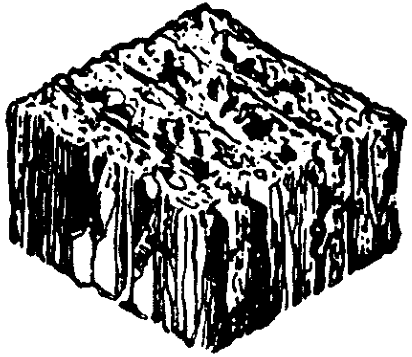
\includegraphics[width=4cm]{../pic/czhx1-ch3-1}
        \caption{显微镜下看到的木材的结构}\label{fig:3-1}
    \end{minipage}
    \qquad
    \begin{minipage}[b]{7cm}
        \centering
        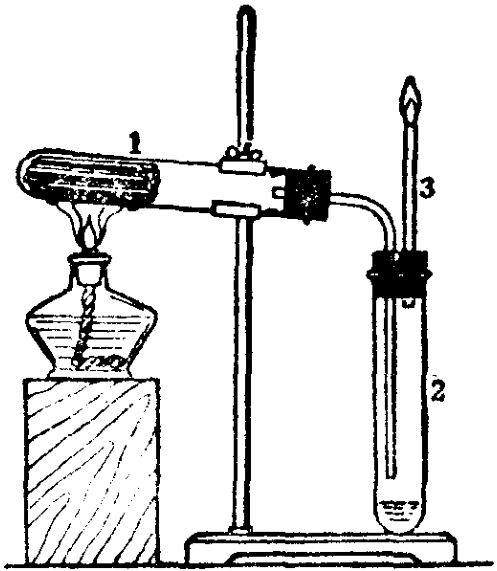
\includegraphics[width=4cm]{../pic/czhx1-ch3-2}
        \caption{木材的干馏}\label{fig:3-2}
    \end{minipage}
\end{figure}

木炭是怎样制成的呢?让木材在隔绝空气的条件下加强热,可以制得木炭。

\begin{shiyan}
    图 \ref{fig:3-2} 是制取木炭的简单装置。

    往试管 1 里放入一些木条(或锯末),给试管加热,
    观察木条发生的变化以及试管 1 靠近塞子的地方和试管 2 的底部发生的现象。
    把火移近尖口管 3 的尖端,观察发生的现象。

    等木条充分变黑以后,移去酒精灯,卸下试管,从试管 1 里取出一根制得的木炭,
    另外取一根小木条,分别用火点,观察发生的现象。为什么?
\end{shiyan}

从上面的实验可以看到,让木材隔绝空气加热,木条逐渐碳化,制得木炭,
除生成黑褐色的叫做木焦油的油状液体外,还生成可以燃烧的叫做木煤气的气体。

\begin{wrapfigure}[11]{r}{5cm}
    \centering
    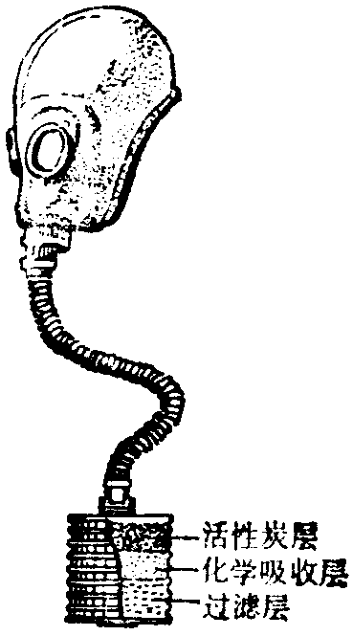
\includegraphics[width=3cm]{../pic/czhx1-ch3-3}
    \caption{防毒面具}\label{fig:3-3}
\end{wrapfigure}

让木材、煤等含碳的物质隔绝空气加强热的过程,叫做\zhongdian{干馏}。

活性炭 活性炭呈黑色粉末状或颗粒状。在隔绝空气的情况下给木炭加强热,并且不断地通入水蒸气,
除去沾附在木炭表面的油质,使管道畅通,来增加木炭的总表面积。经过这样加工的木炭叫做活性炭。
把其它含碳的物质(如核桃壳、椰子壳等)干馏,然后在高温下用水蒸气处理,也可制成活性炭。

活性炭有很强的吸附性能,可以用来净化各种气体和液体。
例如,防毒面具的滤毒罐(图 \ref{fig:3-3}) 就利用活性炭来吸附毒气而使纯净的空气通过;
制糖工业就利用活性炭来除去糖浆里的色素。在居民用水和工业用水的过滤器里,可用活性炭来除去发生臭味的物质。

焦炭 焦炭是一种浅灰色的多孔性固体,质地坚硬。
把烟煤进行干馏,可制得焦炭,同时制得煤气、氨气和煤焦油。
焦炭可用作还原剂和生产水煤气。焦炭还可用于冶金工业上。例如冶炼生铁就需要大量焦炭。


\begin{xiti}

\xiaoti{用什么简单的方法来证明金刚石、石墨和无定形碳是碳元素的同素异形体。}

\xiaoti{区别下列各对名词,并对每一种物质举例说明一种用途。}
\begin{xiaoxiaotis}

    \xxt{石墨、炭黑,}

    \xxt{木炭、活性炭,}

    \xxt{木炭、焦炭。}

\end{xiaoxiaotis}


\xiaoti{在下述两个小实验中选做一个。}
\begin{xiaoxiaotis}

    \xxt{分别燃烧一小片木片和一小段木炭,比较发生的现象。}

    \xxt{用冷碟底在燃着的煤油灯或蜡烛上方收集烟炱。}

\end{xiaoxiaotis}

\end{xiti}

